\section{The WKB Approximation}
The WKB, or Wentzel-Kramers-Brillouin, or semiclassical, or quasiclassical approximation, or the method of steepest descent (used often by mathematicians to find asymptotic behavior of functions in complex analysis!)

\subsection{Motivation for Approximations}
We have three cases in QM where the particle can be solved exactly; the free particle ($V = 0$), the quantum harmonic oscillator ($V = \frac{kx^2}{2}$), and the hydrogen atom ($V = \frac{e^2}{r}$). So in order to study nature, we have to develop the study of approximations. 

We have already studied time-independent perturbation theory. This has applications such as the fine/hyperfine structures of Hydrogen and the Stark/Zeeman effects. The basis idea is that we have some perturbation $V$ much smaller than the typical energy scale of the problem, $\abs{V} \ll \abs{E_n - E_m}$. We then solve for the lowest-order corrections to the energy coming from this small perturbation.

However, this has a problem. Consider for example the Stark effect, where we had the Hamiltonian:
\begin{equation}
    H = -\frac{e^2}{r} - eEz
\end{equation}

\begin{figure}[htbp]
    \centering
    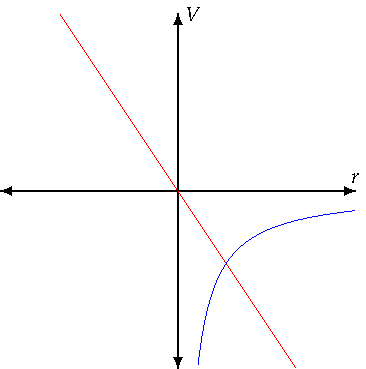
\includegraphics[]{Images/fig-potentialEfieldcoulomb.pdf}
    
    \caption{Potential profile for the Coulomb potential (blue) and the applied external electric field (red).}
    \label{fig-potentialEfieldcoulomb}
\end{figure}

where we treated $-\frac{e^2}{r}$ as the primary Hamiltonian and $-eEz$ as the perturbation. However, consider the phenomena of ionization, where the electric field ionizes hydrogen atoms, freeing the electron. The question: how do we see this phenomena arise in the perturbation theory calculation? We calculate some series $\sum_n c_n g^n$; but no matter to what order we calculate, we don't see the phenomena of ionization. What is the problem? There are some functions which are non-analytic; e.g. $\exp(-\frac{1}{g})$ which cannot be recovered in perturbation theory (as a series expansion of these functions are not meaningful). There are many crucial phenomena attached to this, e.g. ionization, tunneling, alpha decay and so on.

A side note: note that $m_p \sim e^{-1/g}$ - baryonic mass is non-perturbative. So people who use QCD have trouble understanding this phenomena as perturbation theory is pretty useless here.

\subsubsection{Motivation for WKB}
WKB is suited to describe such phenomena. In fact, the potential $V$ is allowed to be large here. The condition we impose is that the potential is slowly varying:
\begin{equation}
    \abs{\dpd{V}{x}} \ll 1
\end{equation}
We discuss phenomena such as ionization, tunneling, (classically describable) highly excited states\footnote{Highly excited states are closer to classical states than the ground states of QM systems.}, which have non-analytic behavior $\exp(-\frac{1}{V})$ which cannot be treated in perturbation theory. 

\subsubsection{Motivation for Adiabatic (Born-Oppenheimer) Approximation}
We consider this approximation when we have slow and fast degrees of freedom. This is often useful for molecular physics. Here we have many nuclei and many electrons. The electron degrees of freedom are extremely fast, with typical frequencies being the electron degrees of freedoms. Comparatively, the protons move very slowly. We can see this as $\frac{m}{M} \ll 1$. It is often used in molecular physics, particle physics and condensed matter physics. The potential can be large, but the key is that there are degrees of freedom moving at different speeds.

\subsubsection{Motivation to Time-Independent PT}
This is useful for treating problems such as radiation and scattering. It is closely related to path integrals in QM, geometric phases, and topological effects. 

\subsection{WKB in 1D}
We have the Schrodinger equation:
\begin{equation}
    -\frac{\hbar^2}{2m}\dod[2]{\psi}{x} + U(x)\psi = E\psi
\end{equation}
if $U \sim \text{Const.}$, then the solutions are known:
\begin{equation}
    \psi \sim e^{\pm i\frac{px}{\hbar}}
\end{equation}
with $\frac{p^2}{2m} = E - U$. We do a change of variables now to write:
\begin{equation}
    \psi(x) = e^{i\frac{S(x)}{\hbar}}
\end{equation}
The logic when developing WKB was that the action $S$ was large for classical physics. Anyways, let us write down what $\psi', \psi''$ are:
\begin{equation}
    \psi' = e^{i\frac{S}{\hbar}}\left(i\frac{S'}{\hbar}\right)
\end{equation}
\begin{equation}
    \psi'' = e^{i\frac{S}{\hbar}}\left(i\frac{S'}{\hbar}\right)^2 + i\frac{S''}{\hbar}e^{i\frac{S}{\hbar}}
\end{equation}
Now let's substitute this back into the SE. No approximations have been made yet here. We're just substituting in an Ansatz:
\begin{equation}
    -\frac{\hbar^2}{2m}\left(-\frac{S'^2}{\hbar^2}\right) - \frac{\hbar^2}{2m}\left(i\frac{S''}{\hbar}\right) + U - E = 0
\end{equation}
now we consider the expansion (which is possible as $S$ is analytic so long as the potential is smooth - but this is quite a deep question. We'll assume the analyticity):
\begin{equation}
    S = S^{(0)} + \frac{\hbar}{i}S^{(1)} + \left(\frac{\hbar}{i}\right)^2S^{(2)} + \ldots
\end{equation}
now, the $S^{(0)}$ in the above is assumed to describe the (large) classical part. We substitute in our expansion and collect terms in various powers of $\hbar$:
\begin{equation}
    -\frac{1}{2m}\left((S^{(0)})'\right)^2 + \frac{i\hbar}{2m}(S^{(0)})'' + E - U - \frac{2}{2m}(S^{(0)})' \frac{\hbar}{i}(S^{(1)})'
\end{equation}
The terms to order $\hbar^0$ give us:
\begin{equation}
    [(S^{(0)})']^2 = 2m(E - U)
\end{equation}
And the terms to order $\hbar^1$ give us:
\begin{equation}
    \frac{i\hbar}{2m}\left[(S^{(0)})'' + 2(S^{(0)})'(S^{(1)})'\right] = 0
\end{equation}
We can rearrange the order $\hbar^0$ equation to obtain:
\begin{equation}
    (S^{(0)})' = \pm \sqrt{2m(E - U)}
\end{equation}
note $p^2/2m = E - U$, and we therefore obtain:
\begin{equation}
    S^{(0)} = \pm \int_0^x p(x') dx'.
\end{equation} 
So we have successfully generalized our formula for the free particle $\psi(x) = e^{\pm i \frac{px}{\hbar}}$. We can see that when $p(x) = p$ a constant that the above formula reproduces the free particle result. So, we have our first result:
\begin{equation}
    \psi(x) = e^{i\frac{S(x)}{\hbar}} = e^{\pm\frac{i}{\hbar}\int_0^x p(x')dx'}
\end{equation}
We can now calculate $S^{(1)}$ using the second equation:
\begin{equation}
    (S^{(0)})'' = - 2(S^{(0)})'(S^{(1)})'
\end{equation}
since $(S^{(0)})' = \pm p(x)$ and $(S^{(0)})'' = \pm \od{p}{x}$, we find:
\begin{equation}
    (S^{(1)})'  -\frac{(S^{(0)})''}{2(S^{(0)})'} = -\dod{p}{x}\frac{1}{2}\frac{1}{p} = -\frac{1}{2}\dod{\log p}{x}
\end{equation}
Therefore:
\begin{equation}
    S^{(1)} = -\frac{1}{2}\log p(x)
\end{equation}
Therefore:
\begin{equation}
    \psi = e^{i\frac{S^{(0)} - i\hbar S^{(1)}}{\hbar}} = e^{\pm i \int^x \frac{p(x')dx'}{\hbar}}\frac{1}{\sqrt{p(x)}}
\end{equation}
If we look at $\abs{\psi}^2$, we have:
\begin{equation}
    \abs{\psi}^2 \sim \frac{1}{\abs{p(x)}} = \frac{1}{mV(x)}
\end{equation}
if we ask the probability of finding a particle, then:
\begin{equation}
    \abs{\psi^2}dx = \frac{dx}{V(x)} = dt
\end{equation}
If we describe the classical physics for a particle in an oscillator, the particle spends a lot of time near the turning points where the velocity is lowest and not a lot of time in the minimum where the velocity is the highest. We reproduce the classical result! WKB were very happy with this.

We have to ask when this approximation is valid. We have the condition assuming:
\begin{equation}
    \abs{\hbar S^{(1)}}' \ll \abs{(S^{(0)})'}
\end{equation}
and so:
\begin{equation}
    \abs{\frac{1}{2}\dod{p}{x}\frac{\hbar}{p}} \ll \abs{p}
\end{equation}
and so:
\begin{equation}
    \dod{}{x}\left(\frac{\hbar}{p}\right) \ll \abs{\dod{\lambda}{x}} \ll 1
\end{equation}
so our approximation is justified when the wavelength of the particle varies slowly with distance.
